% !TEX program = lualatex
% =============================================================================
% Template LaTeX — Índice de Desconforto de Crédito (IDC)
%
% Compilar com: lualatex -interaction=nonstopmode template.tex (duas passagens)
%
% Uso para novo relatório mensal:
%   1. Copie esta pasta para outputs/report/update-YYYYMM/
%   2. Edite a seção "DADOS DO RELATÓRIO" abaixo
%   3. Substitua os \placeholder{} no corpo pelo conteúdo real
%   4. Compile duas vezes
% =============================================================================

\documentclass[11pt,a4paper]{article}

% --- Geometria (margens idênticas ao DOCX original) ---------------------------
\usepackage[
  a4paper,
  left=30mm,
  right=30mm,
  top=25mm,
  bottom=25mm,
  headheight=14mm,
  headsep=6mm,
  footskip=10mm
]{geometry}

% --- Fonte e codificação (LuaLaTeX / XeLaTeX) ---------------------------------
\usepackage{fontspec}
\usepackage{microtype}

\setmainfont{TeX Gyre Pagella}   % clone de Palatino ≈ Cambria
\setsansfont{TeX Gyre Heros}     % clone de Helvetica ≈ Calibri
% Com MS Office instalado, descomente para fontes originais:
% \setmainfont{Cambria}
% \setsansfont{Calibri}[Scale=0.95]

% --- Português do Brasil ------------------------------------------------------
\usepackage[brazilian]{babel}
\usepackage{csquotes}

% --- Gráficos e tabelas -------------------------------------------------------
\usepackage{graphicx}
\graphicspath{{.}}
\usepackage{booktabs}
\usepackage{array}
\usepackage{caption}
\usepackage{subcaption}

\captionsetup[figure]{
  format=plain, labelformat=simple, labelsep=period,
  labelfont={bf}, textfont=it, name=Figura, skip=0.4\baselineskip
}
\captionsetup[table]{
  format=plain, labelformat=simple, labelsep=period,
  labelfont={bf}, textfont=it, name=Tabela, skip=0.4\baselineskip,
  position=above
}

% Nota de fonte abaixo de figuras e tabelas.
% Para figuras, mantenha a fonte dentro do ambiente figure, imediatamente apos
% \caption{}, para que grafico, legenda e fonte flutuem como um unico bloco.
\newcommand{\fonte}[1]{%
  \par\vspace{0.2\baselineskip}%
  \small\textit{Fonte: #1}\par\vspace{0.8\baselineskip}%
}

% --- Tipografia e layout ------------------------------------------------------
\usepackage{xcolor}
\usepackage{setspace}
\usepackage{titlesec}
\usepackage[all]{nowidow}

\onehalfspacing

\titleformat{\section}{\Large\bfseries}{\thesection}{1em}{}
\titlespacing{\section}{0pt}{1.2\baselineskip}{0.6\baselineskip}
\titleformat{\subsection}{\large\bfseries}{\thesubsection}{1em}{}
\titlespacing{\subsection}{0pt}{1.0\baselineskip}{0.4\baselineskip}
\titleformat{\subsubsection}{\normalsize\bfseries}{\thesubsubsection}{1em}{}
\titlespacing{\subsubsection}{0pt}{0.8\baselineskip}{0.3\baselineskip}

% --- Cabeçalho e rodapé -------------------------------------------------------
\usepackage{fancyhdr}
\pagestyle{fancy}
\fancyhf{}
\fancyhead[L]{\small\itshape \reporttitle}
\fancyhead[R]{\small\itshape FGVcemif / FGV-EAESP}
\renewcommand{\headrulewidth}{0.4pt}
\renewcommand{\headrule}{\hbox to\headwidth{%
  \color{black!25}\leaders\hrule height 0.4pt\hfill}}
\fancyfoot[R]{\thepage}
\renewcommand{\footrulewidth}{0pt}

\fancypagestyle{firstpage}{
  \fancyhf{}
  \fancyfoot[R]{\thepage}
  \renewcommand{\headrulewidth}{0pt}
}

% --- Hiperlinks ---------------------------------------------------------------
\usepackage[unicode=true,colorlinks=true,
  linkcolor=black!70,urlcolor=black!70,citecolor=black!70]{hyperref}

% Campos a preencher — aparecem em vermelho no PDF gerado pelo template
\newcommand{\placeholder}[1]{\textcolor{red!70!black}{\textbf{[#1]}}}

% =============================================================================
%   DADOS DO RELATÓRIO — editar a cada atualização mensal
% =============================================================================

\newcommand{\reporttitle}{Índice de Desconforto de Crédito}

% Período de referência
\newcommand{\mesreferencia}{março de 2026}   % ex.: "fevereiro de 2026"
\newcommand{\mesref}{mar-2026}                        % ex.: "fev-2026"
\newcommand{\mesanterior}{fev-2026}                   % ex.: "jan-2026"
\newcommand{\competencia}{202605}                     % ex.: "202604"
\newcommand{\mespublicacao}{maio de 2026}               % ex.: "abril de 2026"
\newcommand{\proxdivulgacao}{junho de 2026}              % ex.: "maio de 2026"
\newcommand{\mesproximo}{abr-2026}                    % ex.: "mar-2026"

% Datas fixas da série (raramente mudam)
\newcommand{\janelainicio}{jan-2014}   % início da janela exibida do IDC
\newcommand{\seriesinicio}{mar-2011}   % início das séries brutas C, I, Q

\newcommand{\reportsubtitle}{Nota Técnica de Atualização --- Competência \mesreferencia}
\newcommand{\reportdate}{29 de maio de 2026}           % ex.: "29 de abril de 2026"

% Autores
\newcommand{\authorone}{Lauro Gonzalez}
\newcommand{\authortwo}{Rafael Schiozer}
\newcommand{\authorthree}{Matheus L. Carrijo}

\hypersetup{
  pdftitle={\reporttitle},
  pdfauthor={\authorone; \authortwo; \authorthree},
  pdfsubject={Nota Técnica de Atualização do IDC},
  pdfkeywords={crédito, endividamento, Brasil, BCB, FGV}
}

% =============================================================================
\begin{document}
% =============================================================================

% --- Capa ---------------------------------------------------------------------
\begin{titlepage}
  \noindent\hfill
\includegraphics[width=79mm]{logo.png}

  \vspace{18mm}

  \begin{center}
    {\LARGE\bfseries \reporttitle\par}
    \vspace{3mm}
    {\large\itshape \reportsubtitle\par}
  \end{center}

  \vspace{12mm}

  \begin{flushright}
    \large
    \authorone\\[2pt]
    \authortwo\\[2pt]
    \authorthree
  \end{flushright}

  \vfill

  \begin{center}
    \reportdate
  \end{center}
\end{titlepage}
\thispagestyle{firstpage}

% =============================================================================
%   CONTEÚDO — substitua os \placeholder{} pelo texto real do relatório
% =============================================================================

\section{Resumo}

Com a publicação, em \mespublicacao, das Estatísticas Monetárias e de Crédito do
Banco Central do Brasil (competência \competencia), o Índice de Desconforto
de Crédito (IDC) foi recalculado e estendido até \mesreferencia{} --- último mês para
o qual há observação disponível da série de comprometimento de renda das famílias (SGS~29034),
que delimita o horizonte de cálculo do índice.

Em mar-2026, o IDC atingiu 0,954, ante 1,000 em fev-2026, mantendo-se em patamar historicamente elevado (4ª maior leitura da série exibida desde jan-2014). Os três componentes recuaram na margem, mas seus valores normalizados continuaram próximos do extremo superior da escala [0, 1], na qual 1,000 representa a pior posição histórica observada e 0,000 a melhor.

\section{Resultados de \mesreferencia}

\begin{table}[htbp]
  \centering
  \caption{Componentes brutos e valores normalizados do IDC --- \mesref.}
  \label{tab:componentes}
  \begin{tabular}{p{8.0cm}rr}
    \toprule
    Indicador & Valor bruto & Valor normalizado \\
    \midrule
    IDC (média dos componentes normalizados)
      & ---
      & \textbf{0,954} \\
    C --- Comprometimento de renda das famílias com a dívida
      & 29,3\%
      & 0,968 \\
    I --- Inadimplência da carteira de crédito livre PF (90+ dias)
      & 7,0\%
      & 0,938 \\
    Q --- Participação das modalidades onerosas no crédito livre PF
      & 24,8\%
      & 0,955 \\
    \bottomrule
  \end{tabular}
\end{table}

\fonte{Banco Central do Brasil (Estatísticas Monetárias e de Crédito,
divulgação \competencia), elaboração própria.}

Em relação à observação imediatamente anterior --- \textbf{\mesanterior}, quando o IDC
marcava \textbf{1,000} --- o índice recuou
\textbf{0,046~ponto} em \mesref.
A melhora foi disseminada entre os três componentes, com quedas simultâneas em comprometimento de renda, inadimplência e participação das modalidades onerosas.

\begin{itemize}
  \item Comprometimento de renda (C) passou de \textbf{29,6\%} para
    \textbf{29,3\%} (-0,3~p.p.).
    O recuo de 29,6\% para 29,3\% reduziu o componente normalizado C de 1,000 para 0,968. Ainda assim, o comprometimento permanece entre os maiores valores da série bruta (posição 3 em ordem decrescente), indicando alívio marginal, mas sem afastamento relevante da zona de maior desconforto relativo.

  \item Inadimplência (I) recuou de
    \textbf{7,2\%} para \textbf{7,0\%}
    (-0,2~p.p.).
    A inadimplência caiu de 7,2\% para 7,0\%, levando o componente normalizado I de 1,000 para 0,938. Como esse valor normalizado segue próximo de 1,000, a leitura ainda está perto do pior ponto histórico observado, embora a variação mensal sinalize redução do desconforto relativo nesse componente.

  \item Qualidade do crédito (Q) caiu de
    \textbf{25,1\%} para \textbf{24,8\%}
    (-0,3~p.p.).
    A participação das modalidades onerosas passou de 25,1\% para 24,8\%, e o componente normalizado Q recuou de 1,000 para 0,955. O nível continua elevado na comparação histórica, o que sugere que a composição do crédito livre PF permanece concentrada em modalidades relativamente mais custosas, apesar da melhora no mês.
\end{itemize}

Em conjunto, os movimentos de março de 2026 apontam redução mensal do desconforto de crédito das famílias, mas a leitura agregada permanece muito próxima do limite superior da escala histórica. Assim, o IDC indica alívio relativo na margem, não uma normalização ampla das condições de crédito captadas pelos três componentes.

\section{Trajetória do índice}

A Figura~\ref{fig:indice} apresenta a evolução do IDC desde jan-2014 e mostra que,
apesar do recuo em mar-2026, o índice permanece próximo ao topo da escala histórica.
A Figura~\ref{fig:componentes} detalha as séries brutas de comprometimento de renda,
inadimplência e qualidade do crédito, permitindo relacionar a leitura agregada do IDC aos
movimentos observados em cada componente.

\begin{figure}[htbp]
  \centering
  \IfFileExists{index.png}{%
    
\includegraphics[width=\linewidth]{index.png}%
  }{%
    \fbox{\rule{0pt}{6cm}\rule{\linewidth}{0pt}}%
  }
  \caption{Evolução do Índice de Desconforto de Crédito (\janelainicio{} a \mesref).}
  \label{fig:indice}
  \fonte{BCB, elaboração própria.}
\end{figure}

\begin{figure}[htbp]
  \centering
  \IfFileExists{components_raw.png}{%
    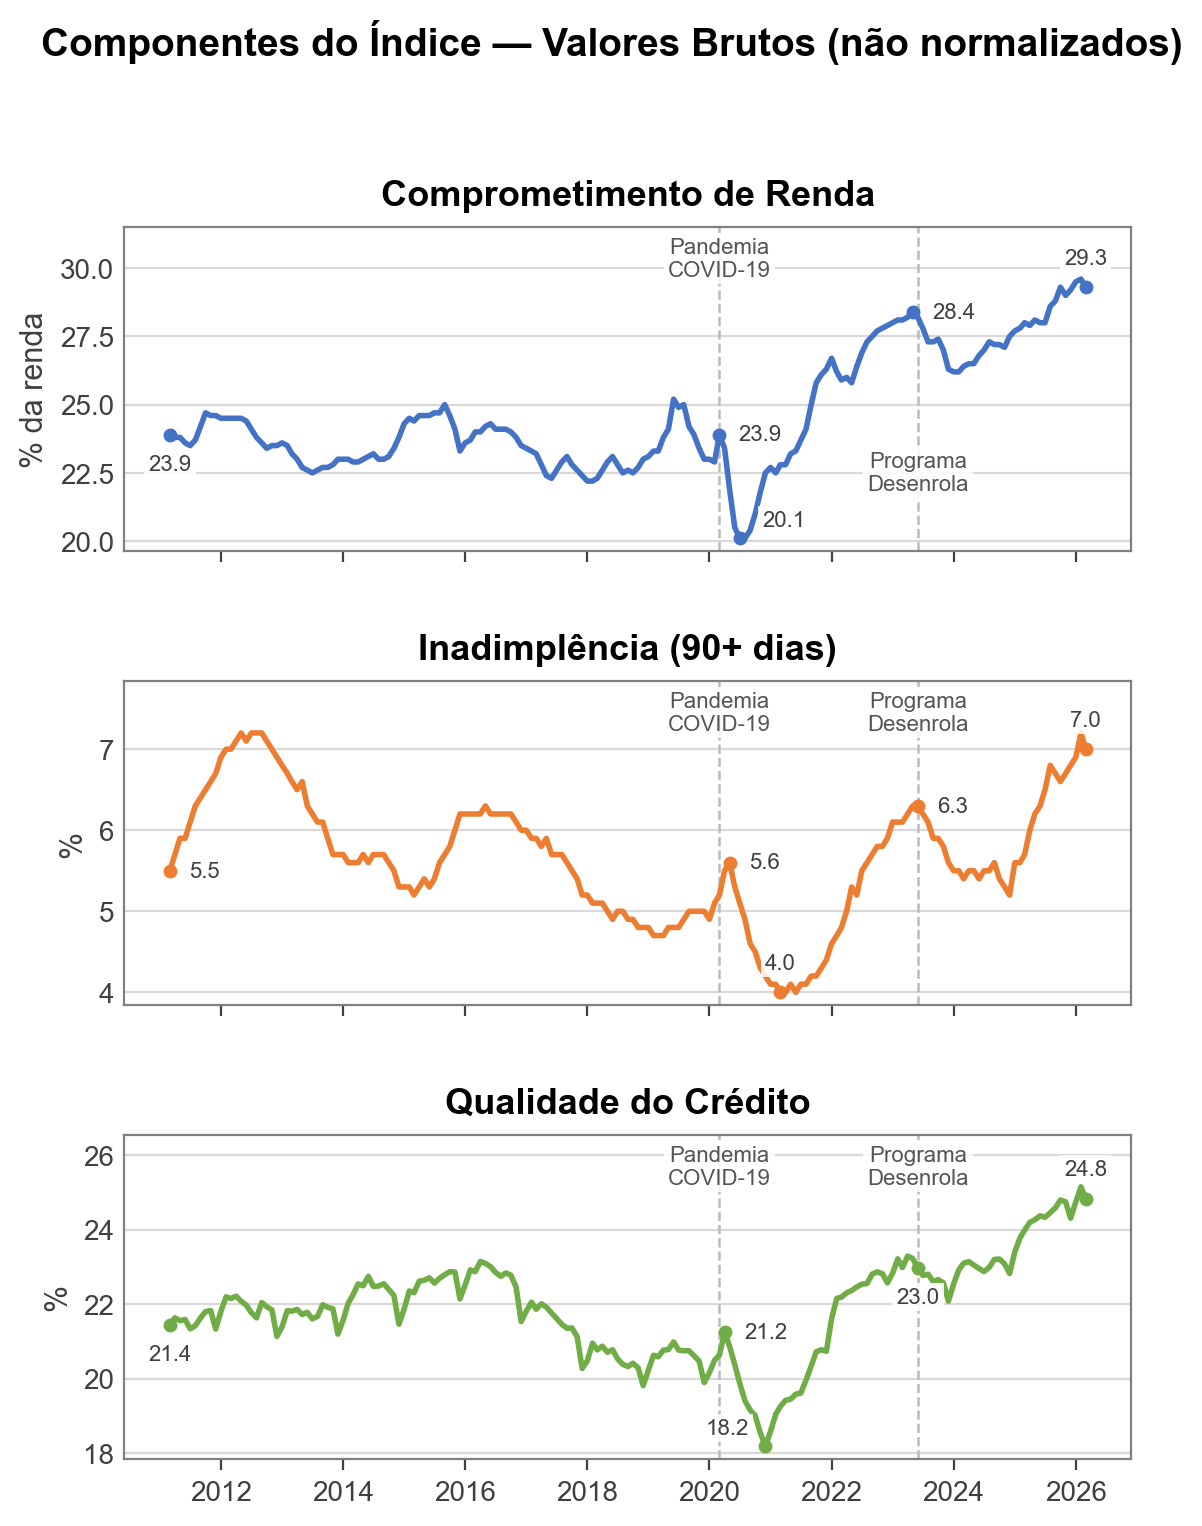
\includegraphics[width=\linewidth]{components_raw.png}%
  }{%
    \fbox{\rule{0pt}{6cm}\rule{\linewidth}{0pt}}%
  }
  \caption{Evolução das componentes brutas C, I e Q (\seriesinicio{} a \mesref).}
  \label{fig:componentes}
  \fonte{BCB, elaboração própria.}
\end{figure}

\section{Próxima atualização}

A próxima atualização do IDC está prevista para a divulgação seguinte das Estatísticas
Monetárias e de Crédito do Banco Central, esperada para \proxdivulgacao.
O índice será estendido para \mesproximo{} caso a série de comprometimento de renda das
famílias (SGS~29034) avance para essa competência.

\section*{Notas}

Sobre o IDC. O Índice de Desconforto de Crédito (IDC) é construído a partir de
três séries do Sistema Gerenciador de Séries Temporais (SGS) do Banco Central do Brasil:
comprometimento de renda das famílias com o serviço da dívida (SGS~29034), inadimplência
da carteira de crédito livre PF --- atrasos superiores a 90 dias (SGS~21112) --- e
participação das modalidades onerosas (cheque especial, SGS~20573; crédito pessoal não
consignado, SGS~20574; cartão de crédito rotativo, SGS~20587; cartão de crédito parcelado,
SGS~20588) no total do crédito livre para pessoa física (SGS~20570). Cada componente é
normalizado pelo método min-max com janela expansiva, a partir de \seriesinicio; o índice
é exibido a partir de \janelainicio, após o período de aquecimento da janela, e corresponde
à média simples dos três componentes normalizados, contido no intervalo [0,~1]. Por
construção, o IDC mede a posição relativa do mês corrente em relação ao histórico observado
pelo índice. O relatório de divulgação está disponível em
\url{https://eaesp.fgv.br/producao-intelectual/indice-desconforto-credito-idc}.

Citação recomendada. Gonzalez, L.; Schiozer, R.; Carrijo, M.~L.
\textit{Índice de Desconforto de Crédito (IDC).} FGVcemif/FGV-EAESP\@.

\end{document}
